\svnidlong
{$HeadURL: $}
{$LastChangedDate: $}
{$LastChangedRevision: $}
{$LastChangedBy: $}

\odachapter{Getting started with OpenDA}

\begin{tabular}{p{4cm}l}
\textbf{Contributed by:} & \\
\textbf{Last update:}    & \svnfilemonth-\svnfileyear\\
\end{tabular}

\section{Introduction}
\oda is a generic environment for data assimilation tasks like parameter calibration and measurement filtering. It provides a platform that allows an easy interchange of algorithms and models.

It is a modular framework, containing methods and tools that can be used for a wide range of applications. By offering the data assimilation software as a separate component, the cost of applying data assimilation methods in one's project is reduced. At the same time, it allows new developments in the field of data assimilation to quickly spread to all applications that might benefit from it.

We assume that the reader is familiar with computational modeling, and with the principal aspects of data-assimilation: the distinction between off-line and on\-line methods, the statistical framework used, the notions of deterministic and stochastic models, and the general structure of filtering methods. 

\section{Installation}
The first thing that needs to be taken care of is the installation of \oda. Please read the appropriate installation page to see how that is done and whether it's done properly. We offer installation instructions for Linux, Mac and Windows.

\subsection{OpenDA installation for Linux users}
\textbf{Note about csh}

At the moment, scripts for csh and related shells are not included with the \oda distribution. It is possible to use \oda in conjunction with for instance tcsh, but you will have to convert the scripts yourself.

\textbf{Note about GNU C Library}

All native components of \oda are compiled for both 32-bit and 64-bit versions of Linux. For 32-bit systems a GLIBC version 2.4 or higher is needed, for the 64-bit version 2.7 or higher. If you have an older version of GLIBC, you need to compile the libraries yourself. It is important to remove all .so files in the lib directory before building. 

\textbf{Step-by-step installation}

\begin{itemize}
\item
Ensure that Java version 1.6 or higher is installed on your computer. You can check which version is installed through the java -version command. We have tested our software with the jre from SUN. The easiest way to install Java is often with the package manager that comes with your distribution (e.g. APT, yum for Red Hat-, dpkg for Debian- or YaST for SUSE-related distributions).
\item
Download \oda from www.openda.org. There is a script available to perform this download: \href{http://www.openda.org/docu/openda_2.1/doc/usedoc/openda_checkout_sf.sh}{openda\_checkout\_sf.sh}
\item
Extract the \oda distribution file to the desired location on your computer. On some Linux systems unzip$/$ark is not installed by default, in that case try the package manager again.
\item
A number of system variables need to be set before \oda can be run. The first variable that should be set is 
\$OPENDADIR. This variable should point to the bin directory of your \oda installation. For example:
    export OPENDADIR$=$myhome$/$openda$/$bin
		
The other variables are set by the script settings\_local.sh in the directory \$OPENDADIR. This script will try to call a local script with machine specific settings \\
\$OPENDADIR$/$settings\_local\_$<$hostname$>$.sh. You must create this script yourself.

Copy the settings\_local\_base.sh file to a new file named settings\_local\_$<$hostname$>$.sh in your \$OPENDADIR (unless that file already exists). You can check your hostname using the hostname command. Then edit that file: enable the relevant lines and change the values of the environment variables.

For Linux there is a default local settings script that might work out of the box for your system. You can use this script by
    . \$OPENDADIR$/$settings\_local.sh linux.
\item
Most convenient is to have the variables set automatically. Add the following two lines to the .bashrc file in your home directory:

export OPENDADIR$=<$bindir$>$, with $<$bindir$>$ the location of the bin directory of your \oda installation.

. \$OPENDADIR$/$setup\_openda.sh

Note that the '.' is significant in the latter of these lines.
\end{itemize}

\subsection{OpenDA installation for Mac users}
\textbf{Step-by-step installation}

\begin{itemize}
\item Ensure that Java version 1.6 or higher is installed on your computer. You can check which version is installed through the java -version command.
\item Download the \oda distribution from www.openda.org.
\item Extract the \oda files to the desired location on your computer.
\item A number of system variables need to be set before \oda can be run. The first variable that should be set is \$OPENDADIR. This variable should point to the bin directory of your \oda installation. For example:

export OPENDADIR$=/$myhome$/$openda$/$bin.

The other variables are set by the settings\_local.sh script in the \$OPENDADIR directory. This script will attempt to call the local script with machine specific settings \$OPENDADIR$/$settings\_local\_$<$hostname$>$.sh. You must create this script yourself.

Copy the settings\_local\_mac.sh file to a new file named settings\_local\_$<$hostname$>$.sh in your \$OPENDADIR directory (unless that file already exists). You can check your hostname using the hostname command. Then edit that file: enable the relevant lines and change the values of the environment variables.

The default local settings script might work out of the box for your system. You can use this script by typing:

. \$OPENDADIR$/$settings\_local.sh mac.
\item Most convenient is to have the variables set automatically. Add the following two lines to the .bashrc file in your home directory:

export OPENDADIR$=<$bindir$>$, with $<$bindir$>$ the location of the bin directory of your \oda installation.

. \$OPENDADIR$/$setup\_openda.sh

Note that the '.' is significant in the latter of these lines.
\end{itemize}

\subsection{OpenDA installation for Windows users}
\textbf{Note about 64-bit systems}

Windows XP is a 32-bit operating system, but some versions of Windows Server, Windows Vista and Windows 7 are 64-bit operating systems and can install the 64-bit version of Java. All native components of \oda are currently compiled for 32-bit versions of Windows only. If you need these native components on a 64-bit system, you have two options:
\begin{itemize}
\item Install a 32-bit version of Java.
\item Compile the native libraries on your machine, see \ref{dc:build:windows}.
\end{itemize}

\textbf{Step-by-step installation}

\begin{itemize}
\item Ensure that Java version 1.6 or higher is installed on your computer, which you can check by typing java -version on the command-line. In case your Java version is too old, you can download the latest version from www.java.com/download
\item Download \oda from www.openda.org
\item Extract the \oda files to the desired location on your computer.
    Note: \oda does not work when it is installed on a location with a space in the path (like "...My Documents").
\item It is no longer needed to edit the start-up bat scripts, as in previous versions of \oda.
\item If you use the command line (cmd.exe), then it is probably convenient to add the bin directory within the \oda directory to the PATH environment variable.
\end{itemize}

\section{Using OpenDA}
The next step will be learning how to use \oda. At first, a brief introduction to data assimilation is presented. The next step is an introduction to \oda itself. After these introductions, you should be ready to start \oda, either from the command-line or the graphical user interface (GUI). Some examples are presented to see how it works.

\oda is configured using XML files. For instance, if you would like to use a different calibration algorithm or stochastic observer, or if you would like to couple your own model to \oda, you should provide all necessary settings, file names, variable names etc. to \oda in XML input files. The format of the XML files is specified in XML schemas (.xsd) files that are hosted on the \oda website. The diagrams describing the format of the XML schemas can found there as well. 

\subsection{Introduction to data assimilation}
Data assimilation is about the combination of two sources of information - computational models and observations - in order to utilize both of their strengths and compensate for their weaknesses.

Computational models are available nowadays for a wide range of applications: weather prediction, environmental management, oil exploration, traffic management and so on. They use knowledge of different aspects of reality, e.g. laws of physics, empirical relations, human behavior, etc., in order to construct a sequence of computational steps, by which simulations of different aspects of reality can be made.

The strengths of computational models are the ability to describe$/$forecast future situations (also to explore what-if scenarios), in a large amount of spatial and temporal detail. For instance weather forecasts are run at ECMWF using a horizontal resolution of about 50 km for the entire earth and a time step of 12 minutes. This is achieved with the tremendous computing power of modern day computers, and with carefully designed numerical algorithms.

However, computations are worthless if the system is not initialized properly: "Garbage in, garbage out". Furthermore the "state" of a computational model may deviate from reality more and more while running, because of inaccuracies in the model; Aspects that are not considered or not modeled well, inappropriate parameter settings and so on. Observations or measurements are generally considered to be more accurate than model results. They always concern the true state of the physical system under consideration. On the other hand, the number of observations is often limited in both space and time.

The idea of data assimilation is to combine a model and observations, and optimally use the information contained in them.

\begin{itemize}
    \item off-line versus on-line;
    \item combine values: weights needed;
    \item statistical framework, std.error;
    \item deterministic versus stochastic models;
    \item noise model;
    \item data-assimilation on top of model.
\end{itemize}

\subsection{Introduction to OpenDA}
\oda is a generic environment for parameter calibration and measurement filtering. It provides a platform, where the interchange of algorithms as well as models can be done easily.

To use \oda, the user needs to prepare some configuration files, in which the information about the data assimilation components is specified. In general, there are three main data assimilation components: stochastic model, stochastic observer, and algorithm. In addition, another component may be specified to configure how \oda output will be stored. The \oda software makes use of the XML (Extensible Markup Language) format for the configuration files.

A number of configuration files are required to provide all necessary information about the \oda application. In general, the user needs to provide one main configuration file and a number of configuration files describing each data assimilation component. The main configuration file contains references to the other components’ configuration files.

The explanation of each configuration file is given below.

\begin{itemize}
    \item Main configuration file (XML schema: openDaApplication.xsd)
    \item In the main configuration file, the \oda java class names, working directories and configuration-file names of all the used data assimilation components are specified.
    \item Stochastic observer \\
		In this configuration file, the user specifies the observation data used in the application as well as the information about its uncertainty.
    \item Algorithm \\
		In this configuration file, the user specifies the input parameters required by the data assimilation or parameter calibration algorithm being used.
    \item Stochastic Model \\
		In this configuration file, the user specifies the model related information.
\end{itemize}

\oda defines certain interfaces, which standardize how different components of \oda communicate with each other. For the model component, \oda defines two levels of interface: the model instance interface and the stochastic model instance interface. The model instance interface defines functionality which a (deterministic) model should implement. On the other hand, the stochastic model instance interface defines the stochastic extension of the deterministic model.

In order for a model to work within \oda, the model should be extended by implementing these interfaces. This is usually called wrapping the model. There are at least five ways one can wrap a model. The first way is to write the model code from scratch in Java and deliberately design the code to match \oda's requirements. The distribution of \oda contains several of such models. Those are small (toy) models, which are developed to test and illustrate various applications of \oda. The second way is to combine native model code with a wrapping Java extension. In this way, we keep the computation core of the model in its original code while extending it with a \oda wrapper. The third way is to write a model in Java, which implements only the model instance interface, and to use the existing Stochastic Black Box model utilities for its stochastic extension. The Black Box model utilities are various functions in \oda for implementing the required interfaces, which are generic and independent from the actual model. Making use of these utilities reduces the work one has to do to wrap a model. The fourth way is like the third one, but the computation core of the model uses the native code. The fifth way is the simplest method to wrap a model: a full black box model. In this way, one only needs to write several functions which read and$/$or write input and output files of the model. Once these methods are ready, one can simply use the Black Box model utilities to create a complete stochastic model extension required for a data assimilation application. While it is the easiest way to implement, an application based on the Black Box wrapper is the most computationally expensive. This is because the communication between the model and other \oda components is performed through writing and reading files.

The configuration files for the stochastic model depend on the type of model. For the toy models which are installed by default with \oda, there is only one model-configuration file needed. On the other hand, three configuration files are required for black-box models: the wrapper configuration, the model configuration, and the stochastic-model configuration. In the wrapper configuration file, the user needs to provide generic information about the model like aliases used to describe the model, the execution steps of the model’s relevant executable, and about input-output Java classes used by \oda to communicate with this model. In the model configuration, specific information of the particular model is given. The stochastic-model configuration file contains the information about vector specifications and may also contain information about the uncertainty of the model. For the DLL-based models, the configuration files needed depend on the choices made by the programmers of the \oda wrapper. In principle, they will require configuration files, where users can specify all the four data assimilation components mentioned above. 

\subsection{Starting OpenDA}
\textbf{Starting OpenDA on Windows}

Run the oda\_run\_gui.bat batch file to open the \oda GUI. Optionally the path to the oda-file can be supplied as an argument, which will open that \oda configuration. The location of your system's Java Runtime Environment can be specified through -jre "path\_to\_jre".

\textbf{Starting OpenDA on Linux$/$Mac}

Run oda\_run.sh \-gui to open the \oda GUI. Optionally the path to the oda-file can be supplied as an argument, which will open that \oda configuration.

\subsection{OpenDA examples}
You can find examples in the examples directory.

\chapter{Developers' corner}
For people who want to (or have to) start from the \oda source code, the Developers' corner is added. The developers' corner is split in two parts: a Java section and a native section. The term native is used for parts of the source code that need to be compiled to a specific platform (Linux, Mac or Windows), formerly known as the Costa PSE.

\section{Building Java sources}
The OpenDA Java source code is located in the core/java directory of the source distribution, but when building everything, ant can be run from the OpenDA root directory (it will use the build.xml file located there).

\oda software consists of four different modules. The first module is the core module, which contains the core of the \oda software. The three other modules are named after the conceptual components of data assimilation: models, observers, and algorithms. Each of these modules contain all programs and files related to the respective data assimilation component. The core module contains programs, which interface the other three modules. Modules for larger models with concrete applications are stored separately.

Native libraries, written e.g. in C or Fortran are provided both as source and binaries with \oda. By default the build processes use the binaries. All binaries provided are 32-bit and therefore need a 32-bit version of Java. You can recompile the required native libraries as 64-bit if needed, for which you will need a 64-bit version of Java. For some blackbox-wrappers en small models you may not need any native libraries, so both 32-bit and 64-bit Java can be used.

\section{Installation of Ant}
To build \oda software, a command-line tool called Ant is used. Ant is similar to make, but written in Java, so that it is portable between different platforms. If Ant is not installed on your computer yet, you can download it from ant.apache.org/bindownload.cgi . For Linux users it is probably easier to use their package manager to install Ant. Before installing Ant, please check that a recent 32-bit version of Java is installed (which can be downloaded from www.java.com/download or in case of Linux, installed with the package manager).

\section{Build commands}
For the following description it is assumed that the \oda source is available in a directory named $<$path\_to\_openda$>$/public .
Start by opening a command window (Windows) or a command shell (Linux) and change directory to the \oda main directory.

\subsection{Compiling OpenDA}
From the OpenDA main directory, you can compile all modules at once. Besides compilation there are several other options:
\begin{itemize}
\item ant (without any argument): to show help with list of possible ant arguments (the same as ant help).
\item ant build: to compile OpenDA, make jar files and copy resources. This doesn't generate Javadoc documentation.
\item ant doc: to build Javadoc for all modules and collect this documentation.
\item ant clean: to remove the generated files.
\item ant zip: to compile OpenDA, collect documentation and xml-schemas and create a set of zip files which contain the subversion revision number in the filename as well as in the name of the readme file. This makes it easy to wrap everything for exporting to a website or user. Exports with the same version numbers will extract to the same openda\_$<$version$>$ directory, but new versions can coexist.
\item ant zip-tests: to create zip files for the various test cases. Each case is stored as separate zip file. Each file is named after the case followed by the version number.
\end{itemize}

\subsection{Compiling individual components}
From the module directory, you can compile a single module. Within a module directory the build file has somewhat different options:

\begin{itemize}
\item ant (without any argument): to show help with list of possible ant arguments.
\item ant build: to compile the module, make jar files and copy resources. This doesn't generate Javadoc documentation.
\item ant javadoc: to build Java doc.
\item ant clean: to remove the generated files.
\item ant make-standalone copy required external binaries to the module directory.
\end{itemize}

\subsection{Compiling stand-alone modules}
When providing others with a stand-alone module, you will have to provide other modules your stand-alone module depends upon (if any). The easiest way to achieve this, is by using ant make-standalone (after building all OpenDA modules) in the module directory. This will copy the files needed to the module directory.

\section{Directory structure}
Upon the execution of the command ant build or ant doc , the following folders are created in the main directory:

\begin{itemize}
\item bin: contains all binary files required for running OpenDA. This will be the content of OpenDA distribution file.
\item doc: contains OpenDA documentation, including some examples.
\item xmlSchemas: contains the XML Schema files for the OpenDA configuration files.
\end{itemize}

Each module directory has the following structure:

\begin{itemize}
\item bin: contains all binary files related to the respective module.
\item build: contains the class files resulting from compiling the Java files of the respective module.
\item javadoc: will contain Java documentation files when they are generated by executing ant javadoc on the command-line.
\end{itemize}

\section{Removal of generated files}
To remove the files generated by a build, you can use ant clean on the command-line. From within a module directory, this command will remove the bin, build and javadoc directories, and the MANIFEST.MF file. It does not affect other modules nor the folder bin in the OpenDA main directory. Executing the command line ant clean from the OpenDA main directory will delete the folders bin, doc, and xmlSchemas in the main directory, as well as removing all modules' generated files. Note: to be able to delete files, they cannot be in use (obviously), so close them first.

\section{Native components}

\subsection{Brief introduction to OpenDA native components}
\textbf{Current practice in data assimilation software}

Data assimilation techniques are widely used in various modeling areas like meteorology, oceanography and chemistry. Most implementations of data assimilation methods however are custom implementations specially designed for a particular model. This is probably a consequence of the lack of generic data assimilation software packages and tools. An advantage of these custom implementations is that they are in general very computationally efficient. But the use of custom implementations has a number of significant disadvantages:

\begin{itemize}
\item Costs - The development and implementation of these methods is very time consuming and therefore expensive.
\item Incompatibility - It is very hard to reuse these data assimilation methods and tools for other models than they were originally developed for. 
\end{itemize}
    
\textbf{How OpenDA improves the situation}

The OpenDA project tries to enhance the reuse of data assimilation software by offering a modular framework for data assimilation, containing methods and tools that can be easily applied for general applications. OpenDA is set up in order to be as computationally efficient as possible, without losing its generic properties. The aim is that applications developed with OpenDA have a comparable computational performance as custom implementations.

\textbf{OpenDA offers support for both users and developers of data assimilation methods.}

For users it allows models to be quickly connected to the OpenDA framework and hence to all the methods that are available in OpenDA. For developers, OpenDA offers efficient basic building blocks that save a lot of programming work and at the same time makes the new data assimilation software directly connectable to all OpenDA compliant models.
How OpenDA works
OpenDA provides a generic framework for data assimilation. It is aimed both at model programmers that want to use data assimilation methods and at developers of data assimilation methods.

\textbf{OpenDA for model programmers}

For model programmers, OpenDA provides a rich set of data assimilation methods. To use them, you have to make your model OpenDA compliant. Once your model can interact with OpenDA, all the OpenDA methods are at your disposal.

\textbf{What is OpenDA compliant?}

Making your model OpenDA compliant involves implementing a number of routines that are going to be called from the data assimilation methods. The set of routines that you must implement is called the stochastic model interface. There are other interfaces as well, each one defining a specific entity called a component. You will read more about components in the next section.

\textbf{How OpenDA calls your implementation of the interface routines}

OpenDA connects your implementations of these methods to their standard names. These standard names are used in the implementation of the data assimilation methods. There are provisions for working with black-box models(i.e. models for which you do not have the source code), but this will not be discussed in this document.

\textbf{Providing your observations}

Likewise, your observations must be provided in a OpenDA compliant way. For the observations there is also a set of routines, called the stochastic observer interface. Usually, you will not implement the interface but convert your observations to a format that can be handled by the standard OpenDA implementation of the stochastic observer component.

\textbf{OpenDA for developers of data assimilation methods}

For developers of data assimilation methods, OpenDA offers a platform for quickly building data assimilation methods that can be used from a wide range of models. OpenDA provides various sets of routines that can be used as building blocks. Such a set is called a component. You will read more about components in the section Components.

\textbf{Routines to interact with models}

First of all, OpenDA specifies a set of routines to interact with the model to which the data assimilation must be applied. Each OpenDA compliant model implements these routines (otherwise it will not be OpenDA compliant). The specification of this set of routines is called the stochastic model interface.

\textbf{Routines to interact with observations}

A second set of routines that is essential for data assimilation methods comprises routines to interact with the observations. These include routines to retrieve values and routines to retrieve meta-information.

\textbf{Basic building blocks}

Finally, there are various sets of basic building blocks (e.g. for handling vectors, matrices and time). These interact seamlessly with the other OpenDA components to let you construct data assimilation methods with a minimum of coding.

\section{Basic concepts of the OpenDA native components}

\subsection{The overall goals}

The overall goal of OpenDA is to provide a toolbox with data assimilation capabilities which may be added easily to existing computational models:

\begin{itemize}
\item OpenDA should be applicable to a wide range of existing computational models.
\begin{itemize}
\item complex, large-scale models should be supported as well as small scale test-models;
\item the models may be implemented using various programming languages, particularly Fortran, C/C++, Java;
\item the models may use parallel computing.
\end{itemize}
\item It should be easy to get started, and one should quickly get initial results.
\item One must be able to achieve good performance for large-scale models.
\end{itemize}

\subsection{The overall philosophy}

\begin{figure}[H]
\center
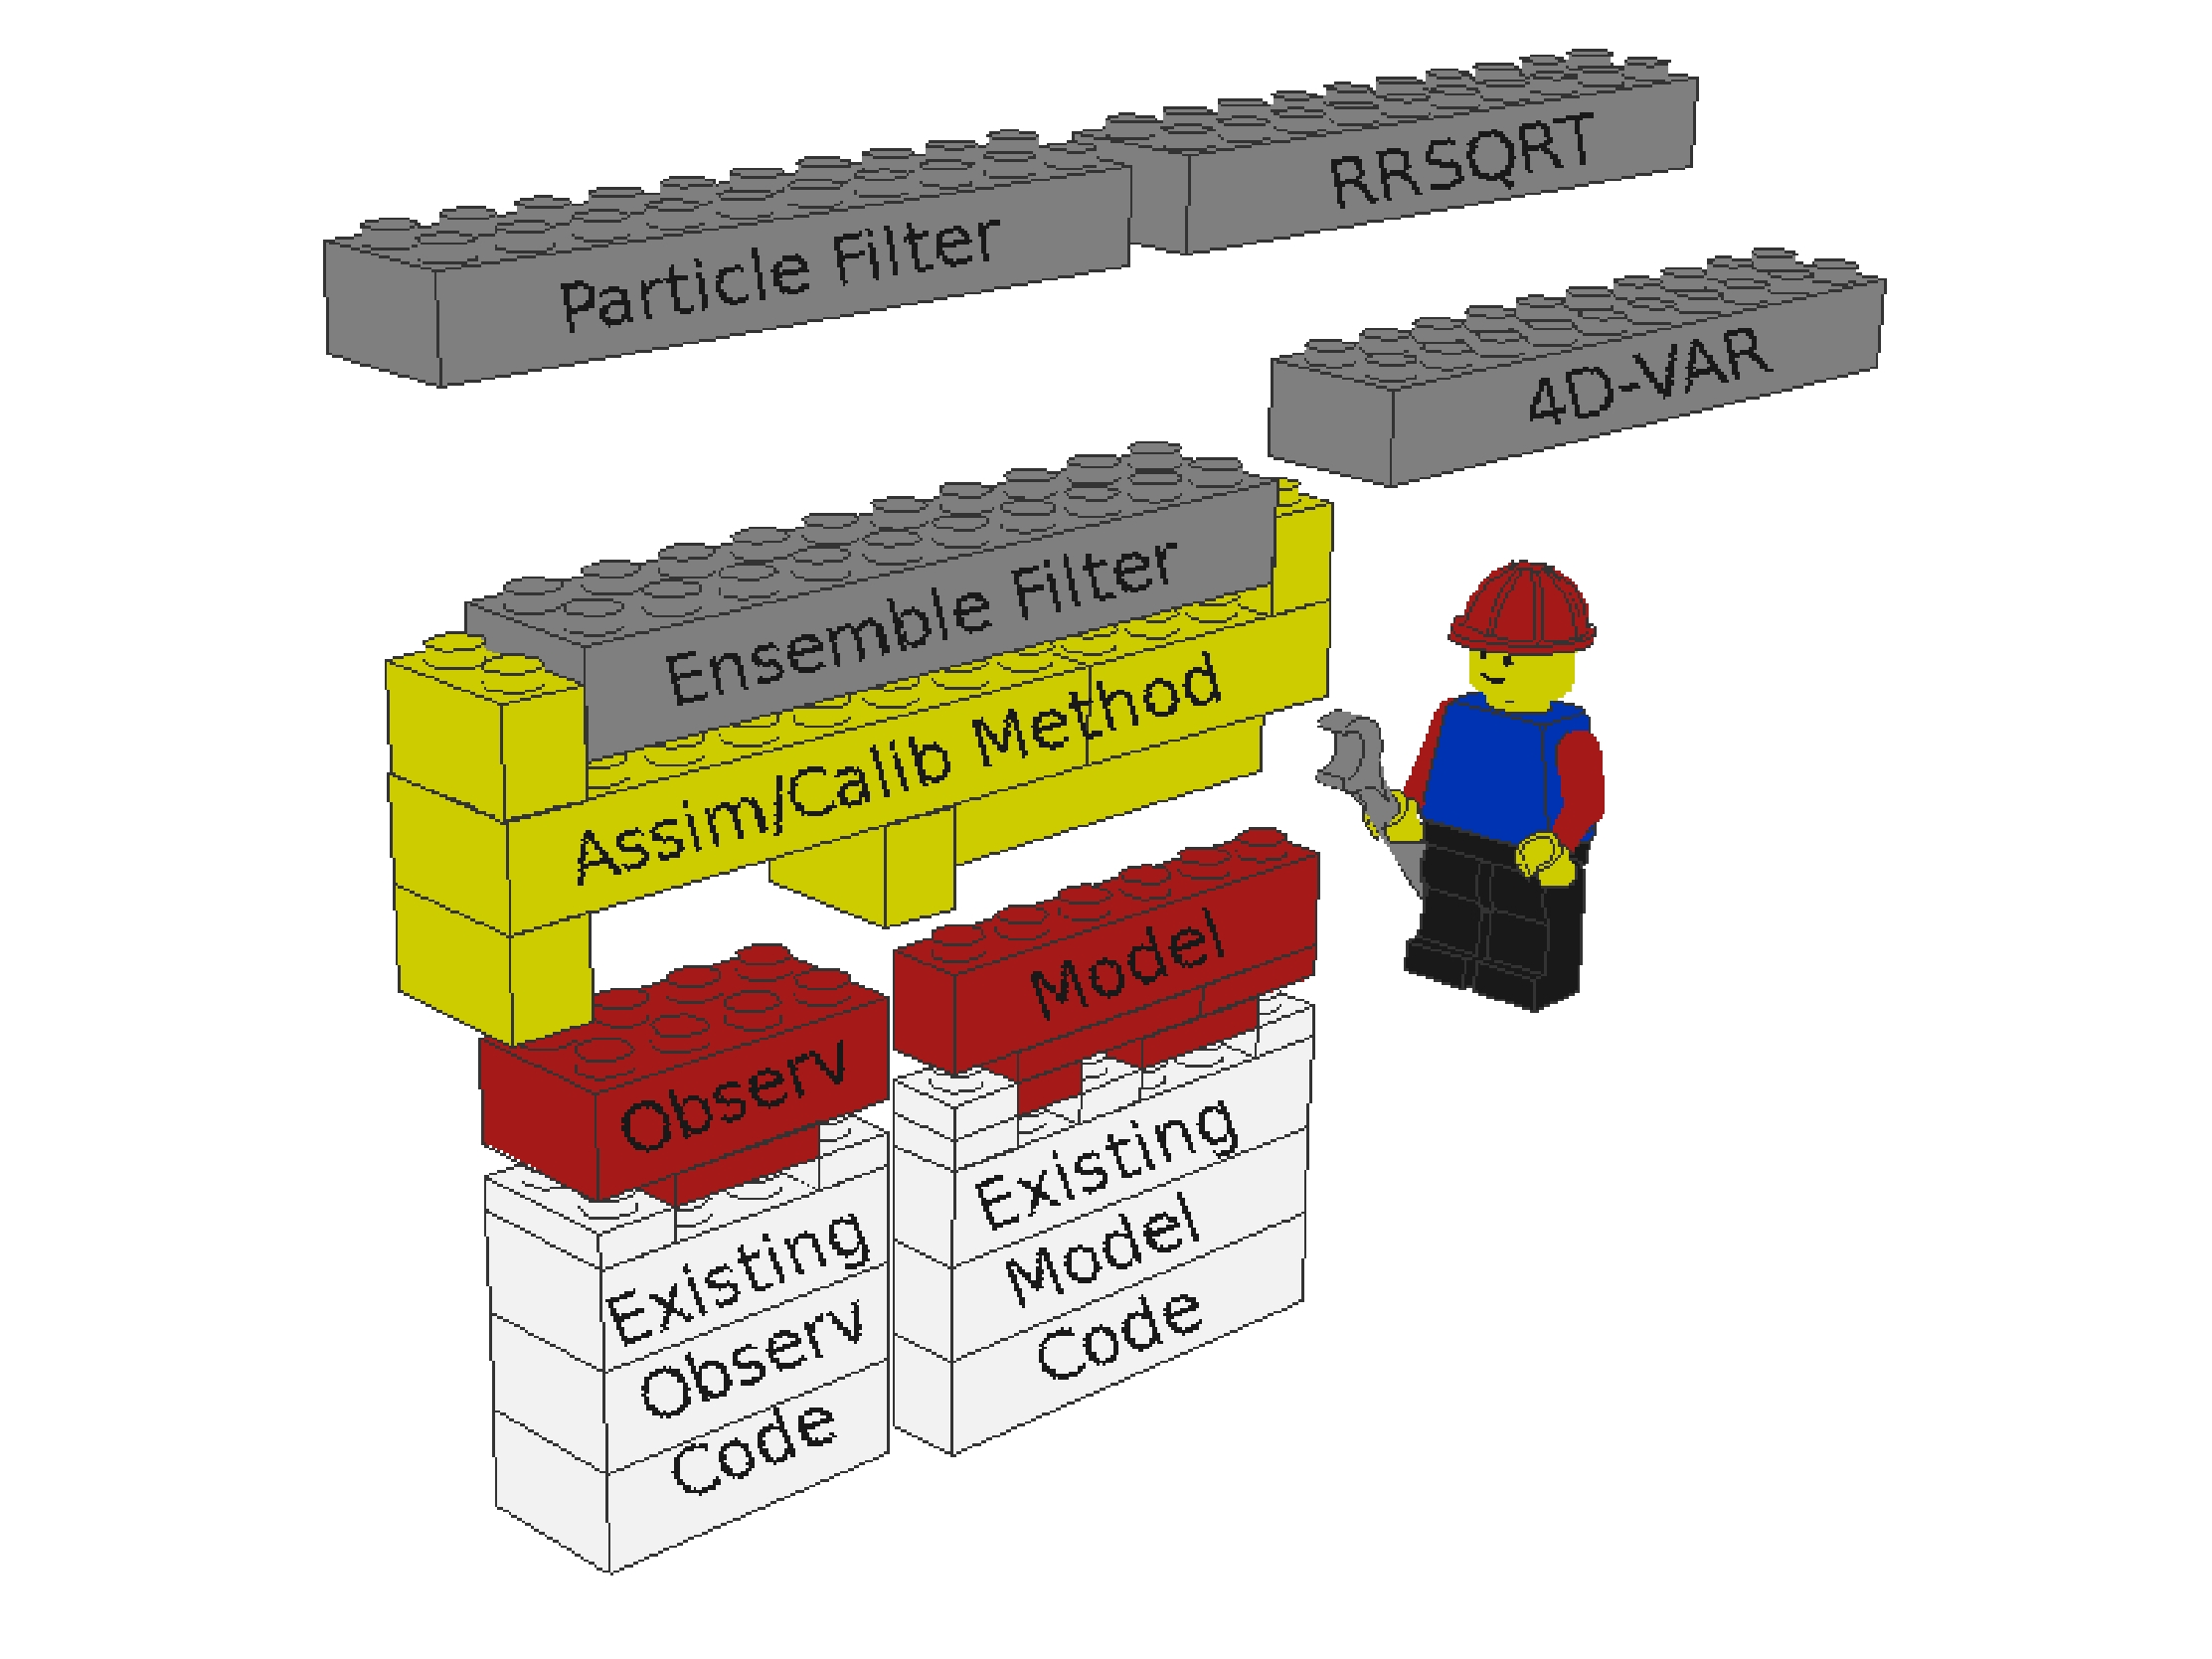
\includegraphics[width=1.0\textwidth]{getting_started/figures/legocomponents2.png}
\caption{Basic design of the OpenDA system. Model and observation components (red/white bricks) are plugged into the core of the OpenDA environment (yellow bricks), and can then exploit the available data-assimilation methods (grey bricks).}
\label{fig:legoblocks}
\end{figure}

The basic design philosophy of OpenDA is illustrated in figure \ref{fig:legoblocks}. The key elements in this picture are:

\begin{itemize}
\item a deterministic or stochastic model (red/white bricks);
\item a collection of observations (red/white bricks);
\item several data assimilation procedures (the grey bricks);
\item the core of the OpenDA-system that connects the different building blocks (the yellow bricks).
\end{itemize}

The figure intends to illustrate a number of important points:

\begin{enumerate}
\item in OpenDA, data assimilation is implemented on top of existing model software;
\item the model and available observations need to be packaged in an appropriate way;
\item the different parts of the complete application are strongly separated from each other.
\end{enumerate}
    

Other aspects, which are not yet illustrated in figure \ref{fig:legoblocks} are:

\begin{enumerate}
\item different "model builders" are provided for quickly packaging existing models and for combining separate models into larger ones;
\item techniques from object orientation are used for providing a basic framework that may be optimized for efficiency.
\end{enumerate}

In OpenDA two components are defined: the OpenDA model component and the OpenDA stochastic observer component. There can be multiple instances of each of these components, each with their own set of data. The set of routines to manipulate the data is called the interface of the component. (Note: the terminology used in OpenDA with respect to object orientation is described in the paragraph about OO terminology).

OpenDA defines the interface of the OpenDA model component. This consists of the list of methods/routines that a model must provide. Examples are "perform a time-step", "deliver the model state", or "accept a modified state". This interface of the model component is visualized through the shape of the empty space in the yellow bricks in the figure above.

Usually, existing model code does not yet provide the required routines, and certainly not in the prescribed form. Therefore some additional code has to be written to convert between the existing code and the OpenDA model components interface. This is illustrated in the figure using red and white bricks: the white bricks stand for the original model code, whereas the red bricks concern the wrapping of the model in order to provide it in the required form.

OpenDA similarly prescribes the interface of the OpenDA observation component. This is visualized using a second empty space in the yellow bricks in the Lego figure. For using OpenDA for your model you must fill in this part, by wrapping the existing code for manipulation of your observations and providing it in the required form.

The data assimilation algorithms in the Lego figure cannot (yet) be seen as instances of another component. For now they are merely routines that implement different data assimilation techniques with the elements provided by OpenDA as the building blocks (models, observations, state vectors etc.). There is however a convergence to a fixed form, a more or less standardised argument list for data assimilation algorithms, such that eventually these may be turned into a well-defined component.

The basic design of OpenDA may seem disadvantageous at first, because it appears to require additional programming work in comparison to an approach where data assimilation is added to a computational model in an ad-hoc way. This is usually not the case. Most of the work in restructuring of the existing model code is needed in an ad-hoc approach too. This is because data assimilation itself puts requirements on the way in which the model equations are implemented in software routines: one must be able to repeat a time step, to adjust the model state, to add noise to forcings or the model state, and so on, which is often not true for computational models that are not implemented with data assimilation in mind.

The basic design does have a huge advantage over an ad-hoc approach for adding data assimilation to an existing program. It is that the different aspects of a data assimilation algorithm are clearly separated. The algorithmics of the precise Kalman filtering algorithm used are separated from the noise model, which in turn may be largely separated from the deterministic model and the processing of observations. This makes it easy to experiment with different choices for each of the parts: adjusting the noise model, adding observations, testing another data assimilation algorithm and so on. This is the major benefit of using the OpenDA approach.

\subsection{Contents of the OpenDA toolbox}

The yellow part in figure \ref{fig:legoblocks} provides the infrastructure needed for connecting generic model and observation components to generic data assimilation methods. We go into the contents of this part in order to gain a better insight in the structure and working of the OpenDA system.

The non-Java components of OpenDA are implemented using non-object oriented programming languages, particularly using Fortran and C. (One reason for this is to avoid difficulties when connecting model software that is written in Fortran and C, another motivation is the experience with Fortran and C of the original developers). However, OpenDA does use ideas from object orientation. In particular the following terminology is used:

\begin{itemize}
	\item An "object" is in OpenDA a variable in a computer program that cannot be manipulated directly, but only through the operations that are defined for it. 
	\item A "class" is the specification of a kind of objects. Objects are instantiations of the class to which they belong. The specification of a class describes both the data (properties, attributes) that objects of the class contain as well as the operations that may be performed. 
	\item The term "(software) component" is used in OpenDA to indicate classes which may involve a large amount of functionality. This concerns the "OpenDA model component" and the "OpenDA (stochastic) observer component". 
	\item The "interface" of a class or a component is the set of routines that may be used to manipulate their instantiations. 
	\item An "OpenDA application" consists of a main program plus all the components, classes and other routines used. It may be packaged into a single executable, may be implemented using dynamic link libraries, or may be implemented in other forms as well. 
\end{itemize}

Whereas the current OpenDA software and documentation often uses the word "component", Wikipedia ("Component based software engineering", "Class (computer science)") suggests that "class" would be more appropriate in most cases, with exceptions for the model and observer components. We suggest to adhere to the terminology introduced here.

\begin{tabular}{l l}
\textbf{OO Language} &	\textbf{OpenDA}\\
String s1, s2; &	CTA\_String s1, s2;\\
char cstr$[$100$]$; &	char cstr[100];\\
S1 = new String; &	CTA\_String\_Create(\&s1);\\
s2 = new String; &	CTA\_String\_Create(\&s2);\\
s1.Set("hello "); &	CTA\_String\_Set(s1,"hello ");\\
s2.Set("world"); &	CTA\_String\_Set(s2,"world");\\
s1.Conc(s2); &	CTA\_String\_Conc(s1, s2);\\
s1.Get(cstr); &	CTA\_String\_Get(s1, cstr);\\
free(s1); &	CTA\_String\_Free(s1);\\
free(s2); &	CTA\_String\_Free(s2);\\
\end{tabular}

Illustration of the use of object orientation in the OpenDA native components: objects are instantiations of OpenDA-defined classes, are represented by object handles, and are manipulated using OpenDA-defined functions for the class.

As an example we consider the support for strings in OpenDA. A class CTA\_String is provided for them. It is a simple container for character strings, which is primarily introduced to shield the difficulties of sharing text strings between Fortran and C. The operations provided for OpenDA strings are to create a new instance, set its value, concatenate strings, retrieve its value, and cleanup a string when it is not needed anymore. A piece of code using this class is presented in the table above.

Another basic class is the OpenDA time class, which provides a uniform way of handling time. The class registers a time span (interval) and optionally contains a time step attribute. It may be extended in a future version with various time scales and representations, time zones, etc..

A third basic building block is the OpenDA vector class, which contains a dimension (length), the data type of the vector elements (equal for all elements), and the values of the vector elements. An advantage of incorporating a vector class in OpenDA is that it provides a generic entity on which data assimilation algorithms can be based, without unnecessarily restricting oneself to the actual data type being used. Further, one can choose to provide different implementations (derived classes) of the vector class, for instance a distributed vector (for parallel computing, sparse vector (if a significant amount of zeros may occur, or using an optimized BLAS version.

An important class in the OpenDA toolbox is the OpenDA tree. It is a generic class for grouping and structuring of data. It may be compared to a "struct" in C or derived type in Fortran. One notable difference is that a OpenDA tree is a dynamic entity: additional items may be added at run-time, with the names of the items provided as string arguments to the creation routines. Therefore a OpenDA tree may also be compared to a file system; nodes contain OpenDA trees (like directories), and leafs contain other OpenDA objects (like files).

A special kind (derived class) of OpenDA tree is the OpenDA tree-vector. It is a OpenDA tree that contains only OpenDA vectors as leaf elements. Of course it provides all the operations that a OpenDA tree class provides. Further it supports the operations that a OpenDA vector is able to perform. The OpenDA tree-vector is important for instance for describing a model state. In data assimilation one must be able to combine different model states much like vectors can be combined. However, representing the model state by a single vector is a severe restriction for many computational models. It is preferable to be able to distinguish different parts of the state, and sometimes needed to distinguish elements with different data types. Furthermore the hierarchical nature of the OpenDA tree-vector supports composition of larger models states out of smaller ones as described later on.

OpenDA primarily uses the XML-format for input/configuration-files. There are several facilities for quickly reading such input-files. OpenDA trees (and tree-vectors) may be written to and read from XML-files as well.

Interfaces are defined to the OpenDA classes for use in Fortran and C/C++. An interface for Java is defined separately in the OpenDA project. This allows data assimilation algorithms to be implemented in Java, and be used together with model components made in Fortran and C.

The OpenDA toolbox can be installed on various Linux and Unix-platforms using the well-known Automake facilities. For the Windows platform project files for Microsoft Visual Studio are provided.

\subsection{Data assimilation methods and the OpenDA Application script}

In the examples above OpenDA applications are created by writing a main program and calling OpenDA routines. In many cases it is more convenient to use the OpenDA Application script instead. This is a generic main program that may be configured to use your model, observations, and the requested data assimilation method.

The OpenDA Application script uses an XML-file to create new OpenDA applications. The XML-file defines the three main ingredients:

\begin{itemize}
	\item The OpenDA model component to be used;
	\item the stochastic observer component to be used;
	\item the data assimilation method used.
\end{itemize}

The OpenDA Application script reads this configuration data, initializes the main model and observation components and then starts the data assimilation algorithm. The assimilation algorithm performs the actual work, and finally the Application script shuts down the computation.

Within the field of data assimilation a distinction between off-line and on-line assimilation methods can be made. Off-line data assimilation concerns model calibration, i.e. optimizing the parameters of a model such that the best fit with a set of observations is obtained.

In these methods the initial value of the model state may be considered as an input parameter of the model as well. This links the 3D-VAR and 4D-VAR variational approaches to the off-line methods listed above.

On-line or sequential data assimilation methods consist of a cycle of forecast and analysis steps, where the methods assimilates the data each time that observations become available. Optimal interpolation methods and Kalman filtering methods fall into this class.

\subsection{The OpenDA stochastic model component}

OpenDA uses a fixed form for a model component, in order to provide consistent terminology to both data assimilation methods and model implementers. The general form of a OpenDA model is
$x(t+\Delta t) = M(x(t), p, u(t), w(t))$.
Here x stands for the model state, t represents time, p is a vector of parameters, u concerns the forcings of the model, w is the noise/uncertainty, and M is the model operator. Simpler forms of models are possible, for instance a deterministic model without noise/uncertainty, a model without parameters or without forcings, and so on. Although this does not turn a model into an invalid OpenDA model, it may limit the data assimilation techniques that can be applied.

Data assimilation techniques will have to access the model state. This cannot be done directly. A model may use its own representation of the state. The interface of the OpenDA model component however requires that a model be able to provide a copy of the state in a OpenDA tree-vector, and that linear operations on a state-vector can be performed.

Linear operations on the model state are an important aspect of the interface of the model component because these operations are used frequently in data assimilation algorithms, and because the implementation may be dependent on the actual model that is implemented. For instance a model may require positivity of specific quantities that it computes (e.g. waterdepth in a flow model), such that blindly combining two state-vectors may give inappropriate results. Therefore a more careful combination recipe may be implemented by the model itself. 

\subsection{The use of native model builders}

The idea of OpenDA is to make it simple to get started, but to provide full flexibility as well. This is implemented by providing default implementations where possible, but to also allow redefinition of the OpenDA components.

One place where this idea is given concrete form is in the concept of model builders. A model builder is more or less a template for creating new native model components. It fills in as many of the routines that must be provided, such that setting up a new model component is greatly simplified. Once one is up and running one can then tune the implementation to ones own ideas.

\textbf{The sp-model builder}

The SP model builder ("single processor") can be used to quickly create sequential (non-parallel) model components. This model builder defines choices for the storage and administration of the state vector, model parameters, changes to the forcings, and the noise parameters. With these choices made, a large portion of the methods that must be provided by a model component are provided by the model builder already, and only a few model specific methods have to be filled in.

\textbf{The parallel model builder}

The parallel model builder is meant for computational models that use parallel computing, and which probably must be started in an appropriate way. It is primarily meant for computational models that use MPI, which are based on multiple executables. Parallelization using multi-threading, especially using OpenMP, can often be used in OpenDA using a direct approach, for instance using the sp-builder.

Note that parallelization of data assimilation methods can often be achieved in different ways. A data assimilation algorithm often contains multiple model computations that may be performed in parallel, and each model computation itself may be parallelized too. The former approach to parallelization is called "mode-parallel". This name stems from the term "error modes" that may be used for different model instantiations in certain Kalman filtering algorithms. The latter approach using parallelization of the model computation itself is called "space-parallel", which indirectly refers to the domain decomposition approach. The two approaches may be combined as well, which gives a "mode and space-parallel" approach.

The parallel model builder is primarily concerned with space-parallelization. Mode-parallelization is already provided by the sp-builder ("using OpenDA, you get mode-parallelization for free"). It is provided by the parallel model builder as well, which yields the mode+space parallel approach.

The architecture used by the parallel model builder is to use an SPMD-approach ("single-program, multiple data"), i.e. to start the main OpenDA-application (executable) multiple times. Within the group of processes that is created in this way, the first one acts as the master process. This process performs the data assimilation algorithm. The other processes perform the model computations.

Computational models that use a master-worker approach for their parallelization may fit well into this approach. The master process of the original computational model may be integrated with the OpenDA master process. The subroutines that are required by the OpenDA model components interface may be filled in using the routines of the model's master process. This may be achieved well with the sp-builder.

The parallel model builder is mainly concerned with computational models that are parallelized using a worker-worker approach, e.g. using domain decomposition, where each computational process solves a different part of a global domain.

The routines that are specified in the OpenDA model components interface, like "perform a timestep", are implemented differently in the master and worker processes. In the master process, these routines consist of sending MPI messages to the worker processes, and waiting for the corresponding results. The results are joined together more or less the same as when different sub-models are combined into a composite model.

The worker processes read a configuration file from which they learn about their role in the global computation. Then they go into "worker-mode". This consists of an indefinite loop, waiting for MPI messages, and calling the appropriate model routines. The model routines are implemented just like for a sequential model. One notable difference is that these routines are called in all worker processes simultaneously, such that communication between the workers may be used.

The parallel model builder provides the infrastructure needed for setting up this scheme. It provides the model routines for the master process and the worker mode for the OpenDA main program. The model engineer just has to provide the model routines for the worker processes.

\subsection{The OpenDA stochastic observer component}

In OpenDA an observation is not just a value, but contains all the information available for use in a data assimilation method. This involves for instance information on the measurement error, which may be described by a probability density function. Other aspects of observations are the type of quantity that is observed, the unit, time, grid location, and so on.

The Stochastic Observer is the OpenDA component that holds an arbitrary number of observations. It may be instantiated multiple times.

A stochastic observer may be queried for a selection of the observations that it holds. For instance the observations within a given timespan may be requested, for a selected set of "stations", or that measure a specific quantity. Such a selection may be used to create a new stochastic observer object.

The stochastic observer further takes care of computing predicted values at observation locations. This concerns the observation relation that is used in data assimilation algorithms: the model state is interpolated and/or converted to the observation location and observed quantity. For this the implementation of a stochastic observer must know the structure of a model state vector, the meaning of its components, and the procedures available for spatial and/or temporal interpolation. For this a stochastic observer contains a substantial application dependent part.

OpenDA provides default implementations of the stochastic observer and observation descriptions. In this default implementation observations are stored in an SQLite3 database. The database contains two tables, "stations" and "data" for time-independent and time-dependent information respectively. This default implementation provides a basis for setting up ones own observation component. It should grow over time with features that are relevant to different computational models. 

\section{Building sources}

\subsection{Linux}

This page describes how to build the OpenDA native source code on Linux computers. The source code is located in the core/native directory of the source distribution. On Linux, the native sources are compiled using the GNU Automake system.

Directory scripts of the source distribution contains a script $openda_build_native.sh$ that may be useful to compile the native code. It was tested for Ubuntu 8.04 lts 32-bit only. In this script, you will recognize the steps described below.

\textbf{Building step-by-step}

\begin{enumerate}
	\item The first step is starting the configure script, usually through ./configure (to ensure the script you are starting is the one in the current directory and not another one from the search path). This will detect the configuration of the computer being used and will warn when specific requirements are not met. When all requirements are met, make files will be generated. It is possible to alter the behaviour of the configure script by using command-line arguments. The most important ones are: 
	\begin{itemize}
		\item --help will list all options with some help text.
		\item --prefix=PATH indicates the place the library should be copied to after make install.
		\item --disable-mpi disables MPI.
		\item --with-blas=PATH indicates the location of the BLAS library. By default, an unoptimized BLAS library is used.
		\item --with-lapack=PATH indicates the location of the LAPACK library, an unoptimized LAPACK library is used.
		\item --with-jdk=PATH indicates the location of the Java Development Kit (JDK) if it differs from the value of \$JAVA\_HOME.
		\item --with-jikes=PATH indicates the location of the Jikes Java compiler in case that compiler is to be used. Default: no.
	\end{itemize}
	Do not forget to scan the configure output for warnings. Those are often very informative. 
\item The second step is using make to build (compile and link) the source files.
\item The final step is copying the resulting libraries (and executables) to the place specified using configure's --prefix= command-line argument. This step is activated by make install. 
\end{enumerate}

The Automake system also generated the other usual make options (like make clean ). It is unlikely that you want to remove the libraries and executables you just built, but in case you want to, this is nice to know. 

\textbf{Note about OpenMPI}

There is a known problem with OpenMPI versions 1.3 and 1.4 where an external dependency mca\_base\_param\_reg\_int cannot be found during run-time. This can be avoided by recompiling OpenMPI itself. Use command-line arguments --enable-shared --enable-static when running the config script. 

\subsection{Mac}

This page describes how to build the OpenDA native source code on Mac computers. The source code is located in the core/native directory of the source distribution. On Mac computers, the native sources are compiled using the XCode development environment. 

\textbf{Preliminaries}

\begin{enumerate}
	\item Install XCode.
	\item Install a GFortran compiler that is compatible with your Xcode installation.
	\item Install OpenMPI (the same version as Xcode) with fortran support (--ensable-static --enable-dynamic). and insert the path in front of your \%PATH\% and \%LD\_LIBRARY\_PATH\% variables.
	\item Install a Java Development Kit (JDK).
\end{enumerate}

\textbf{Building step-by-step}

\begin{enumerate}
	\item The first step is starting the configure script, usually through ./configure. This will detect the configuration of the computer being used and will warn when specific requirements are not met. When all requirements are met, make files will be generated. It is possible to alter the behaviour of the configure script by using command-line arguments. The most important ones are: 
	\begin{itemize}
		\item --help will list all options with some help text.
		\item --prefix=PATH indicates the place the library should be copied to after make install.
		\item --disable-mpi disables MPI.
		\item --with-netcdf=PATH indicates the location of the NetCDF library.
		\item --with-jdk=PATH indicates the location of the Java Development Kit (JDK) if it differs from the value of \$JAVA\_HOME.
	\end{itemize}
	Do not forget to scan the configure output for warnings. Those are often very informative. 
	\item Build (compile and link) the source files.
	\item Copy the resulting libraries (and executables) to the place specified using configure's --prefix= command-line argument. 
\end{enumerate}

\subsection{Windows}
\label{dc:build:windows}

This page describes how to build the OpenDA native source code on Windows computers. The source code is located in the core/native directory of the source distribution. The Microsoft Visual Studio solution file is located at core/native/vs2010/OpenDANativeAll.sln .

\textbf{Note about Microsoft Visual Studio and Intel Fortran}

The solution and project files provided are for the following version of the development environment:

\begin{itemize}
	\item vs2010 and Intel Fortran Composer 13 or higher
\end{itemize}

When you use a newer version of mentioned tools, it is fine to upgrade these files to your version. In case you are working from the repository, please do not check in these upgraded files. 

\textbf{Building step-by-step}

\begin{enumerate}
	\item Load the solution file core/native/vs2010/OpenDANativeAll.sln into Microsoft Visual Studio.
	\item Select whether you want to perform a Release build or a Debug build.
	\item Start the build process with Build All.
\end{enumerate}

\textbf{Note about the Intel Fortran library path}

In some installations of Microsoft Visual Studio, the Intel Fortran library path is not added to the library path during the installation (and integration) of Intel Visual Fortran. This will lead to a link error about one or more missing libraries, usually ifconsol.lib,

If this is the case, solve it by either:

\begin{itemize}
	\item Add the lib directory of the Intel Fortran installation to the global library path in Microsoft Visual Studio. This path can be found in Visual Studio menu path Tools/Options/Projects and Solutions/VC++ Directories/Library files.
	\item Add the lib directory of the Intel Fortran installation to the project's (probably libcta's) library path. This path can be found the project's right-click menu: path Properties/Configuration Properties/Linker/General/Additional Library Directories.
\end{itemize}
    
    
